\chapter{Desarrollo del diseño}

El desarrollo de esta solución se basa en el trabajo previamente desarrollado por \textcite{Vargas2023}, quien propuso un modelo de tipo \textit{Hierarchical Temporal Memory }(HTM) para la detección de anomalías en los signos vitales de pacientes en Unidades de Cuidados Intensivos Pediátricos (UCIP). Dicho modelo permite analizar múltiples señales médicas de un paciente de forma conjunta, sin requerir una predefinición del número exacto de variables de entrada.

\begin{figure}[ht]
  \centering
  \includesvg[width=\textwidth, inkscapelatex=false]{Images/ArquitecturaOriginal.svg}
  \captionsetup{justification=centering}
  \caption{Arquitectura del modelo HTM propuesto por Vargas para la detección de anomalías en signos vitales.}
  \label{fig:arquitectura_original}
\end{figure}

Una de las ventajas más destacables del modelo HTM utilizado por Vargas es su capacidad de generalización ante una variabilidad en la cantidad de señales fisiológicas disponibles. En entornos reales de la UCIP, no todos los pacientes cuentan con la misma cantidad de dispositivos de monitoreo. Algunos pacientes, debido a su condición crítica, requieren sensores adicionales de naturaleza más intrusiva, mientras que en otros casos, estos dispositivos se reducen gradualmente a medida que su estado clínico mejora. Además, es frecuente que ciertos sensores se desconecten temporalmente durante procedimientos rutinarios como el baño o la movilización del paciente. Frente a estas variaciones, el modelo HTM mantiene su operatividad, pues no requiere una configuración rígida de entradas, adaptándose así a este contexto clínico dinámico.

No obstante, una de las principales limitaciones del modelo propuesto por Vargas radica en la falta de interpretabilidad de los resultados generados. El sistema es capaz de identificar que una anomalía ha ocurrido, pero no especifica cuál variable o conjunto de variables fisiológicas ha contribuido a dicha detección. Esta característica reduce el valor explicativo del modelo frente al personal clínico, quienes necesitan comprender con claridad qué parámetros vitales están generando la alerta, de tal forma que puedan identificar de manera precisa los sistemas fisiológicos afectados y ajustar oportunamente sus intervenciones, con el objetivo de estabilizar las condiciones fisiológicas del paciente y maximizar las posibilidades de recuperación. En este contexto, un modelo que permitiera identificar con precisión qué factores fisiológicos están teniendo un mayor impacto en el estado clínico del paciente, tendría un valor significativamente superior para la toma de decisiones médicas fundamentadas \parencite{zhang2023interpretable}.

Además, es necesario destacar otra desventaja crítica: el modelo de Vargas identifica como anómalos todos los cambios bruscos en las señales fisiológicas, sin considerar los rangos normales ajustados por edad del paciente. Esta falta de contextualización puede llevar a interpretaciones erróneas. Por ejemplo, incluso cuando un paciente experimenta una mejora clínica y sus parámetros vitales transitan rápidamente desde un estado fuera del rango normal hacia un rango fisiológicamente aceptable, el modelo puede interpretarlo como una anomalía por tratarse de un cambio abrupto. Esta situación puede generar falsas alarmas, provocando interrupciones innecesarias en la atención médica, distracción del personal y, en algunos casos, desgaste en la confianza del equipo clínico hacia el sistema automatizado. En un entorno tan delicado como la UCIP, la precisión de las alertas no solo es deseable, sino crítica.

Por consiguiente, aunque el enfoque propuesto por Vargas representa un avance significativo en la automatización del análisis de signos vitales, este trabajo busca superar dichas limitaciones mediante un rediseño del sistema de detección, empleando una estrategia basada en detección de anomalías en subespacios (\textit{subspace anomaly detection}). Este enfoque permite asociar cada anomalía detectada con un subconjunto específico de las variables fisiológicas de entrada, brindando así mayor interpretabilidad respecto al origen de las anomalías detectadas. Adicionalmente, se incorporan elementos de contextualización clínica, como la edad del paciente, y, con ello, ajustar de forma más precisa el nivel de criticidad asociado a cada alerta generada. De este modo, el sistema no solo identifica la ocurrencia de una anomalía, sino que también asocia de forma explícita el conjunto de variables fisiológicas involucradas en dicha anomalía. Esta capacidad resulta fundamental para facilitar la comprensión clínica del evento, mejorar la toma de decisiones médicas y reducir la incidencia de alertas irrelevantes o poco informativas.

\section{Recolección de información}

Para el desarrollo y validación del sistema propuesto, se contó con registros clínicos reales proporcionados por la Unidad de Cuidados Intensivos Pediátricos (UCIP) del Hospital Militar Central de Bogotá. Estos datos fueron suministrados con el propósito de verificar la efectividad del modelo de detección de anomalías propuesto en un entorno clínico real, respetando los lineamientos éticos y de confidencialidad establecidos por la institución.

El conjunto de datos corresponde a pacientes pediátricos entre 8 y 15 años de edad, monitoreados durante períodos continuos que oscilan entre 16 y 24 horas, con una frecuencia de muestreo de un registro por minuto. Esto permite una granularidad suficiente para capturar tanto tendencias lentas como fluctuaciones rápidas en el estado fisiológico del paciente. En total, se recopilaron aproximadamente 136 horas de registros distribuidos en ocho pacientes, lo que otorga una base representativa y sólida para evaluar la eficacia del método propuesto.

La Tabla~\ref{tab:pacientes} presenta el listado de los pacientes incluidos en el estudio, junto con su edad, diagnóstico médico y la cantidad de horas de monitoreo de signos vitales registradas para cada uno. En total de horas de monitoreo consideradas en el análisis asciende a 122,95 horas.

\captionsetup{justification=centering} % Centra el caption de la tabla
\begin{table}[ht]
  \centering
  \begin{tabular}{
      >{\columncolor[HTML]{E8E8E8}}l
      >{\columncolor[HTML]{FFFFFF}}l
    >{\columncolor[HTML]{FFFFFF}}l l}
    \cellcolor[HTML]{AFB8CC}Id & \cellcolor[HTML]{AFB8CC}Edad & \cellcolor[HTML]{AFB8CC}Diagnóstico Médico & \cellcolor[HTML]{AFB8CC}Horas de monitoreo \\
    Paciente 1                 & 8 años                            & Tumor Pulmonar                             & 23,03 horas                                      \\
    Paciente 2                 & 10 años                           & Infarto Cerebral                           & 16,65 horas                                            \\
    Paciente 3                 & 11 años                           & Tumor Cerebral                             & 16,65 horas                                            \\
    Paciente 4                 & 12 años                           & Septicemia                                 & 16,65 horas                                            \\
    Paciente 5                 & 14 años                           & Choque séptico refractario                 & 16,65 horas                                            \\
    Paciente 6                 & 15 años                           & Cetoacidosis diabética                     & 16,65 horas                                            \\
    Paciente 7                 & 15 años                           & Hipertensión endocraneana                  & 16,65 horas                                            \\
  \end{tabular}
  \caption{Pacientes incluidos en el estudio, diagnóstico y horas de monitoreo registradas.}
  \label{tab:pacientes}
\end{table}

Para todos los registros de pacientes, se cuenta con registro de todos los siguientes signos vitales, con la excepción del paciente 2, para quien únicamente se dispone de datos de FC, SpO\textsubscript{2} y Resp.

\begin{itemize}
  \item \textbf{FC}: Frecuencia Cardíaca, medida en latidos por minuto.
  \item \textbf{SpO\textsubscript{2}}: Saturación de oxígeno en sangre, representada como un valor porcentual.
  \item \textbf{Resp}: Frecuencia Respiratoria, en respiraciones por minuto.
  \item \textbf{ARTs}: Presión Arterial Sistólica, medida en mmHg.
  \item \textbf{ARTd}: Presión Arterial Diastólica, medida en mmHg.
\end{itemize}

Estos parámetros (“FC”, “SpO\textsubscript{2}”, “Resp”, “ARTs” y “ARTd”) constituyen la base principal para evaluar de manera integral el estado hemodinámico y respiratorio del paciente, siendo indispensables para la monitorización en entornos de cuidados intensivos. Si bien se dispone también de registros de la presión arterial media (ARTm), esta magnitud muestra una correlación estadísticamente muy elevada con las presiones sistólica y diastólica, dado que se relaciona directamente con ellas a través de la siguiente fórmula:

\[
  \mathrm{ARTm} \approx \frac{2\,\mathrm{ARTd} + \mathrm{ARTs}}{3}
\]

por lo cual su inclusión aportaría información redundante en el modelo. De igual forma, se cuenta con registros de temperatura corporal en la mayoría de los pacientes; no obstante, como menciona \textcite{Vargas2023}, la temperatura, aunque clínicamente útil en otros contextos, no representa un indicador de alta relevancia para la detección temprana de eventos de deterioro en entornos de cuidados intensivos, donde sus variaciones tienden a ser leves y poco significativas. Por tal motivo, este indicador también fue excluido de las variables de entrada.

Por otro lado, vale la pena resaltar que estos datos recrean varios de los desafíos de la práctica hospitalaria, ya que incluyen lapsos de ausencia ocasionados por desconexiones temporales de los monitores o fallos en la captura de las señales. Dicha heterogeneidad en la disponibilidad y calidad de las mediciones demanda que el sistema sea robusto frente a conjuntos de datos incompletos o intermitentes, tal como ocurre en entornos clínicos.

A continuación, se presenta la tabulación de los signos vitales del paciente 3 a lo largo del tiempo, con el fin de ilustrar gráficamente la presencia de estos periodos de ausencia y la variabilidad en la presencia de ruido en las señales.

\begin{figure}[ht]
  \centering
  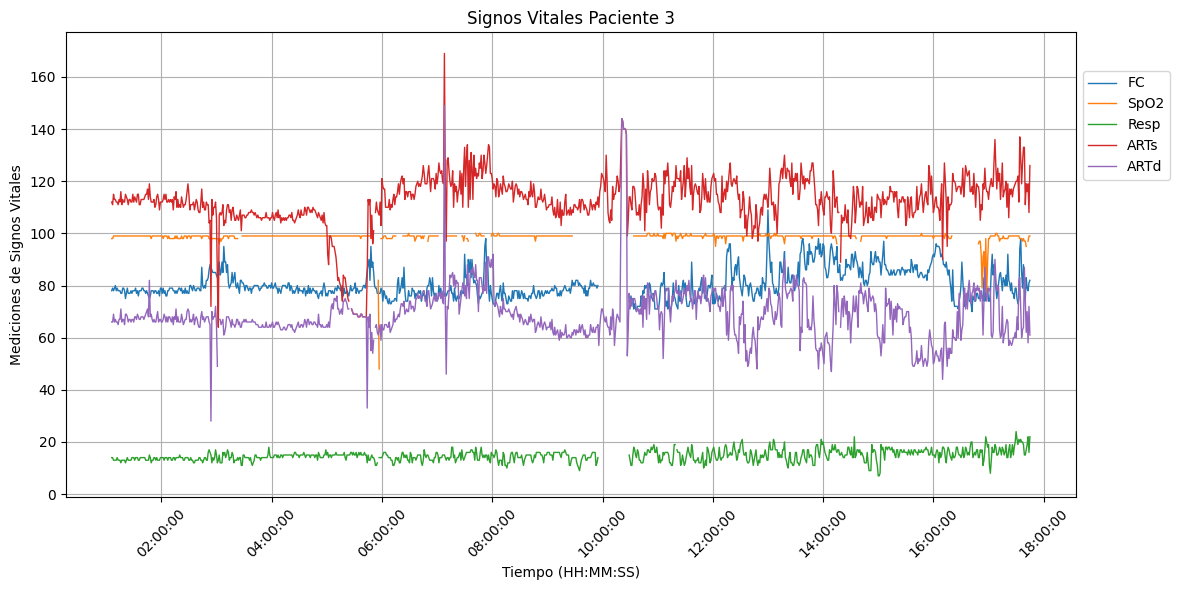
\includegraphics[width=\textwidth]{Images/SignosVitalesPaciente3.png}
  \caption{Evolución temporal de los signos vitales del paciente 3, mostrando periodos de ausencia y ruido en las señales.}
  \label{fig:signos_vitales_paciente3}
\end{figure}

\section{Alternativas de diseño}

En su sección de trabajo futuro, \textcite{Vargas2023} sugiere como alternativa un esquema en el que el sistema de detección de anomalías se componga de tres modelos predictivos HTM independientes, cada uno alimentado por un par de señales altamente relacionadas: uno con presión sistólica y diastólica, otro con saturación de oxígeno e índice de perfusión, y un tercero con frecuencia cardiaca y respiratoria. Según Vargas, esta división permitiría mejorar la interpretabilidad, al concentrar cada motor de alarma en una relación estrecha entre señales que provienen de la misma medición o que presentan alta correlación estadística.

No obstante, aunque esta configuración facilita entender qué par de variables está generando cada alerta, el hecho de limitar la búsqueda de anomalías a parejas predefinidas de señales puede empobrecer la calidad global del análisis. Además, restringir la búsqueda de anomalías únicamente a pares de señales ya altamente correlacionadas o procedentes del mismo monitor puede limitar significativamente la capacidad del sistema para detectar patrones clínicos más complejos que afecten diferentes sistemas coporales. En este sentido, \textcite{Pieroni2023}, al estudiar el uso de distintos modelos de \textit{machine learning} para aplicaciones clínicas, demuestra que considerar un abanico más amplio de parámetros y combinaciones de variables incrementa la capacidad de generalización y el rendimiento predictivo del modelo. Por lo tanto, al analizar un mayor numero de interacciones entre signos vitales, se espera capturar patrones de deterioro clínico que de otro modo pasarían desapercibidos.

A partir de este hecho, este trabajo opta por una visión más amplia que expande el concepto de “análisis por pares” a todas las combinaciones posibles de dos señales de entrada (también conocidas como subespacios bidimensionales). En la arquitectura propuesta, cada una de estas combinaciones alimenta de forma independiente un modelo HTM encargado de detectar comportamientos atípicos en el espacio conjunto de la pareja, con el fin de identificar desviaciones en su correlación que puedan indicar un inicio de deterioro fisiológico o un evento adverso. De esta manera, al analizar cada subespacio 2D, el sistema no solo mejora su interpretabilidad, dado que se asocia cada anomalia a una pareja de dos signos vitales, sino que también captura un rango más diverso de anomalías potenciales, reflejando fielmente las complejas interrelaciones que existen entre los distintos signos vitales en la práctica clínica \parencite{Pieroni2023}.
